% ============================================================
% FINAL REPORT SLIDE: Hybrid Search for Academic Documents
% LaTeX Beamer — Metropolis Dark Theme (~20-25 phút)
% ============================================================
\documentclass[aspectratio=169, 11pt]{beamer}

% ---- Encoding & Language ----
\usepackage[utf8]{inputenc}
\usepackage[T5]{fontenc}
\usepackage{vietnam}

% ---- Theme ----
\usetheme{metropolis}

% ── Dark theme customization ──
\definecolor{primaryDark}{HTML}{0F1B2D}
\definecolor{primaryMid}{HTML}{1A2744}
\definecolor{accentTeal}{HTML}{2DD4BF}
\definecolor{accentBlue}{HTML}{60A5FA}
\definecolor{accentOrange}{HTML}{FB923C}
\definecolor{accentPurple}{HTML}{A78BFA}
\definecolor{accentRed}{HTML}{F87171}
\definecolor{textWhite}{HTML}{F1F5F9}
\definecolor{textLight}{HTML}{CBD5E1}
\definecolor{textMuted}{HTML}{94A3B8}
\definecolor{boxBg}{HTML}{1E293B}
\definecolor{highlightRow}{HTML}{134E4A}
\definecolor{codeGreen}{HTML}{6EE7B7}
\definecolor{codePurple}{HTML}{C4B5FD}

% Apply dark Metropolis
\setbeamercolor{normal text}{fg=textWhite, bg=primaryDark}
\setbeamercolor{alerted text}{fg=accentOrange}
\setbeamercolor{example text}{fg=accentTeal}
\setbeamercolor{title separator}{fg=accentTeal}
\setbeamercolor{progress bar}{fg=accentTeal, bg=primaryMid}
\setbeamercolor{progress bar in head/foot}{fg=accentTeal, bg=primaryMid}
\setbeamercolor{progress bar in section page}{fg=accentTeal, bg=primaryMid}
\setbeamercolor{frametitle}{bg=primaryMid, fg=white}
\setbeamercolor{block title}{fg=white, bg=accentBlue!70!black}
\setbeamercolor{block body}{fg=textWhite, bg=boxBg}
\setbeamercolor{block title alerted}{fg=white, bg=accentRed!70!black}
\setbeamercolor{block body alerted}{fg=textWhite, bg=boxBg}
\setbeamercolor{block title example}{fg=white, bg=accentTeal!60!black}
\setbeamercolor{block body example}{fg=textWhite, bg=boxBg}
\setbeamercolor{itemize item}{fg=accentTeal}
\setbeamercolor{itemize subitem}{fg=accentBlue}
\setbeamercolor{enumerate item}{fg=accentTeal}
\setbeamercolor{footline}{fg=textMuted, bg=primaryMid}
\setbeamercolor{page number in head/foot}{fg=accentTeal}
\setbeamercolor{section in toc}{fg=textWhite}

\setbeamertemplate{section in toc}[sections numbered]
\metroset{progressbar=frametitle}

% ---- Packages ----
\usepackage{amsmath, amssymb}
\usepackage{graphicx}
\graphicspath{{./}{../images/}}
\usepackage{tikz}
\usetikzlibrary{arrows.meta, positioning, shapes.geometric, calc, backgrounds, fit, decorations.markings}
\usepackage{listings}
\usepackage{booktabs}
\usepackage{multirow}
\usepackage{hyperref}
\usepackage{array}
\usepackage{colortbl}
\usepackage{pifont}
\newcommand{\cmark}{\ding{51}}  % checkmark
\newcommand{\xmark}{\ding{55}}  % xmark

% Code listing style
\lstdefinestyle{codestyle}{
    basicstyle=\ttfamily\scriptsize\color{textWhite},
    keywordstyle=\color{codePurple}\bfseries,
    stringstyle=\color{codeGreen},
    commentstyle=\color{textMuted}\itshape,
    backgroundcolor=\color{primaryMid},
    frame=single,
    rulecolor=\color{accentTeal!40},
    breaklines=true,
    showstringspaces=false,
    tabsize=2,
}
\lstset{style=codestyle}

% ---- Metadata ----
\title{Building a Hybrid Search System\\for Academic Documents using Elasticsearch}
\subtitle{Kết hợp Keyword Search, Semantic Search và Hybrid Search}
\author{
  \texorpdfstring{
    \textbf{GVHD:} PGS.TS Thoại Nam\\[0.2cm]
    {\small
    Dương Gia An -- 2470293 \quad
    Trịnh Sơn Lam -- 2470287 \quad
    Nguyễn Thanh Huyền -- 2570416
    }
  }{Group 11}
}
\institute{Đại học Bách khoa TP.HCM --- Khoa KH \& KT Máy tính\\CO5135 --- Big Data (HK252)}
\date{Tháng 5, 2026}
\titlegraphic{
\includegraphics[height=1.2cm]{hcmut.png}}

% ============================================================
\begin{document}

% ============================================================
% PHẦN MỞ ĐẦU: Title, Contribution, TOC
% ============================================================

% ── SLIDE 1: Title ──
\begin{frame}[plain]
    \begin{center}
        \vspace*{0.05cm}
        
\includegraphics[height=1.0cm]{hcmut.png}
        \vspace*{0.15cm}
        
        % Đóng khung cả tên seminar và phần tiếng Việt phụ đề
        {\color{accentTeal}\setlength{\fboxrule}{1.2pt}\setlength{\fboxsep}{7pt}\fbox{%
            \begin{minipage}{0.80\textwidth}
                \centering
                {\large \bfseries BUILDING A HYBRID SEARCH SYSTEM\\FOR ACADEMIC DOCUMENTS USING ELASTICSEARCH}
                
                \vspace*{0.1cm}
                {\small \color{textWhite} Xây dựng Hệ thống Tìm kiếm Kết hợp cho Tài liệu Học thuật sử dụng Elasticsearch}
            \end{minipage}%
        }}
    \end{center}
    
    \vspace*{0.05cm}
    
    % Góc phải giữa: Tên giảng viên & sinh viên
    \begin{flushright}
        {\footnotesize \color{textLight}
        \begin{tabular}{r}
            \textcolor{textMuted}{GVHD:} PGS.TS Thoại Nam \\[0.08cm]
            \textcolor{textMuted}{Sinh viên thực hiện:} \\
            Dương Gia An --- 2470293 \\
            Trịnh Sơn Lam --- 2470287 \\
            Nguyễn Thanh Huyền --- 2570416
        \end{tabular}
        \hspace*{0.5cm}
        }
    \end{flushright}
    
    \vspace*{\fill}
    
    % Dưới cùng: Thông tin trường, khoa, môn học và ngày tháng
    \begin{center}
        {\scriptsize \color{textMuted}
        Đại học Bách khoa TP.HCM --- Khoa KH \& KT Máy tính --- CO5135 --- Big Data (HK252) \\
        Tháng 5, 2026
        }
    \end{center}
\end{frame}

% ── SLIDE 2: Contribution ──
\begin{frame}{Phân công công việc}
\begin{center}
\renewcommand{\arraystretch}{1.3}
{\small
\begin{tabular}{c l p{6.8cm} c}
\toprule
\textbf{STT} & \textbf{Thành viên} & \textbf{Đóng góp} & \textbf{Tỷ lệ} \\
\midrule
1 & Dương Gia An & System Architecture, Elasticsearch Indexing, Search Pipeline, Evaluation \& Benchmarking & 33.33\% \\
\hline
2 & Trịnh Sơn Lam & Data Preprocessing, GPU Embedding Pipeline, Ground Truth Labeling & 33.33\% \\
\hline
3 & Nguyễn Thanh Huyền & Theoretical Background, Evaluation Analysis, Final Report Compilation & 33.33\% \\
\bottomrule
\end{tabular}
}
\end{center}
\end{frame}

% ── SLIDE 3: TOC ──
\begin{frame}{Nội dung trình bày}
\begin{columns}[T]
\begin{column}{0.48\textwidth}
\tableofcontents[sections={1-4}]
\end{column}
\begin{column}{0.48\textwidth}
\tableofcontents[sections={5-8}]
\end{column}
\end{columns}
\end{frame}
         % Title, Contribution, TOC
% ============================================================
% CHƯƠNG 1: Giới thiệu — Bối cảnh, Bài toán, Mục tiêu, Dataset, Schema
% ============================================================
\section{Giới thiệu}

% ── SLIDE 4: Bối cảnh ──
\begin{frame}{Bối cảnh và Động lực}
\begin{columns}[T]
\begin{column}{0.50\textwidth}

\begin{alertblock}{Thực trạng}
{\footnotesize Mỗi ngày thế giới tạo ra \textbf{2.5 quintillion bytes} dữ liệu. Phần lớn là \textbf{phi cấu trúc}: văn bản, ảnh, video, bài báo...}
\end{alertblock}

\vspace{0.05cm}

{\footnotesize \textbf{Các kho dữ liệu học thuật:}}
\begin{itemize}\itemsep0pt \parskip0pt \parsep0pt
    \item \textcolor{accentBlue}{\textbf{arXiv}}: 2.4+ triệu bài báo
    \item \textcolor{accentOrange}{\textbf{Google Scholar}}: 380+ triệu bài
    \item \textcolor{accentPurple}{\textbf{PubMed}}: 36+ triệu bài
\end{itemize}

\end{column}
\begin{column}{0.46\textwidth}

\begin{exampleblock}{Vấn đề hiện tại}
{\footnotesize
\begin{itemize}\itemsep0pt \parskip0pt \parsep0pt
    \item \textbf{Keyword Search}: chỉ khớp từ vựng, ``car'' $\neq$ ``automobile''
    \item \textbf{Semantic Search}: hiểu ngữ nghĩa nhưng mất chính xác cho thuật ngữ chuyên ngành
    \item[$\Rightarrow$] Cần \textcolor{accentTeal}{\textbf{Hybrid Search}}!
\end{itemize}
}
\end{exampleblock}

\vspace{0.05cm}

\begin{block}{Ba thế hệ tìm kiếm}
{\footnotesize
\begin{enumerate}\itemsep0pt \parskip0pt \parsep0pt
    \item \textcolor{accentBlue}{\textbf{Lexical}} (1970s): Đối khớp từ khóa
    \item \textcolor{accentOrange}{\textbf{Semantic}} (2018): Hiểu ngữ nghĩa
    \item[\textcolor{accentTeal}{$\star$}] \textcolor{accentTeal}{\textbf{Hybrid}} (2022+): Kết hợp cả hai
\end{enumerate}
}
\end{block}

\end{column}
\end{columns}
\end{frame}

% ── SLIDE 5: Bài toán ──
\begin{frame}{Bài toán nghiên cứu}
\begin{block}{Problem Statement}
{\small Cho truy vấn $q$, tìm và xếp hạng tài liệu liên quan từ kho \textbf{1.2M+ bài báo khoa học}, kết hợp:}
\begin{itemize}\itemsep0pt \parskip0pt \parsep0pt
    \item \textcolor{accentBlue}{\textbf{Keyword search}} (BM25) --- khớp từ vựng chính xác
    \item \textcolor{accentOrange}{\textbf{Semantic search}} (dense vectors) --- hiểu ngữ nghĩa
    \item \textcolor{accentTeal}{\textbf{Hybrid search}} (RRF) --- kết hợp song song thông qua RRF
\end{itemize}
\end{block}

\vspace{0.1cm}

\begin{columns}[T]
\begin{column}{0.46\textwidth}
\begin{alertblock}{Keyword Search thất bại}
{\footnotesize
Query: ``methods to detect fake images''\\
$\to$ Không match ``deepfake detection''\\
\textbf{0 từ khóa chung!}
}
\end{alertblock}
\end{column}
\begin{column}{0.50\textwidth}
\begin{alertblock}{Semantic Search thất bại}
{\footnotesize
Query: ``ViT-B/16 fine-tuning''\\
$\to$ Model hiểu chung chung ``vision model''\\
\textbf{Mất precision cho exact terms!}
}
\end{alertblock}
\end{column}
\end{columns}
\end{frame}

% ── SLIDE 6: Mục tiêu ──
\begin{frame}{Mục tiêu dự án}
\begin{enumerate}
    \item \textcolor{accentTeal}{\textbf{Hybrid Search System}}: Xây dựng hệ thống tìm kiếm kết hợp keyword search + semantic search trên \textbf{Elasticsearch 8.12}

    \vspace{0.15cm}
    \item \textcolor{accentBlue}{\textbf{GPU Embedding Pipeline}}: Thiết kế pipeline nhúng vector cho \textbf{1.2M+ tài liệu} với GPU acceleration

    \vspace{0.15cm}
    \item \textcolor{accentOrange}{\textbf{Microservice Architecture}}: Triển khai kiến trúc \textbf{Dual-Index} trên Docker (FastAPI + React)

    \vspace{0.15cm}
    \item \textcolor{accentPurple}{\textbf{Evaluation}}: Đánh giá bằng \textbf{NDCG@10, MRR@10} với 30 test queries

    \vspace{0.15cm}
    \item \textcolor{accentTeal}{\textbf{Web Application}}: Giao diện tìm kiếm với 3 chế độ (keyword search, semantic search, Hybrid search), bộ lọc năm/category
\end{enumerate}
\end{frame}

% ── SLIDE 7: Dataset ──
\begin{frame}{Dataset --- arXiv Paper Abstracts}
\begin{columns}[T]
\begin{column}{0.50\textwidth}

\begin{block}{Nguồn dữ liệu}
{\small
\begin{itemize}\itemsep0pt \parskip0pt \parsep0pt
    \item \textbf{Nguồn}: Kaggle (Cornell University)
    \item \textbf{Tổng}: 2.7M+ bài báo, 4.8GB raw JSON
    \item \textbf{Lọc}: Chỉ lấy \texttt{cs.*} (Computer Science)
    \item \textbf{Kết quả}: \textcolor{accentTeal}{\textbf{1,203,108}} bài báo CS
\end{itemize}
}
\end{block}

\vspace{0.1cm}

\begin{exampleblock}{Quy trình làm sạch}
{\scriptsize
Streaming đọc $\to$ Lọc \texttt{cs.*} $\to$ Loại JSON lỗi $\to$ Chuẩn hóa text $\to$ Trích xuất năm $\to$ Xuất JSONL
}
\end{exampleblock}

\end{column}
\begin{column}{0.46\textwidth}

\begin{block}{Thống kê mô tả}
\centering
\renewcommand{\arraystretch}{1.0}
{\small
\begin{tabular}{l l}
\toprule
\textbf{Chỉ số} & \textbf{Giá trị} \\
\midrule
Tổng bài báo & 1,203,108 \\
Thể loại CS & 40 subcategories \\
Khoảng thời gian & 1993--2024 \\
Title trung bình & $\sim$10 từ \\
Abstract trung bình & $\sim$150 từ \\
Dung lượng raw & 4.8 GB \\
Dung lượng JSONL & 12 GB \\
\bottomrule
\end{tabular}
}
\end{block}

\end{column}
\end{columns}
\end{frame}

% ── SLIDE 8: Data Schema ──
\begin{frame}{Cấu trúc dữ liệu --- 6 Fields}
\centering
\renewcommand{\arraystretch}{1.1}
{\small
\begin{tabular}{l l l p{6cm}}
\toprule
\textbf{Field} & \textbf{ES Type} & \textbf{Vai trò Search} & \textbf{Mô tả} \\
\midrule
\texttt{id} & \texttt{keyword} & Exact match & Mã định danh arXiv duy nhất \\
\texttt{title} & \texttt{text} & BM25 (boost $\times$2) & Tiêu đề bài báo \\
\texttt{abstract} & \texttt{text} & BM25 + Embedding & Tóm tắt nội dung \\
\texttt{categories} & \texttt{keyword} & Filter/Aggregation & Mã thể loại (cs.AI, cs.LG...) \\
\texttt{authors} & \texttt{text} & BM25 & Danh sách tác giả \\
\texttt{year} & \texttt{keyword} & Filter & Năm xuất bản \\
\bottomrule
\end{tabular}
}

\vspace{0.1cm}

\begin{columns}[T]
\begin{column}{0.48\textwidth}
\begin{block}{\texttt{text} field}
{\footnotesize Phân tích tokenization, lowercase, stop-word removal $\to$ \textbf{Inverted Index} $\to$ Full-text search (BM25)}
\end{block}
\end{column}
\begin{column}{0.48\textwidth}
\begin{block}{\texttt{keyword} field}
{\footnotesize Lưu nguyên bản, không phân tích $\to$ \textbf{Doc Values} $\to$ Exact-match filter, aggregation}
\end{block}
\end{column}
\end{columns}
\end{frame}
    % Bối cảnh, Bài toán, Mục tiêu, Dataset, Schema
% ============================================================
% CHƯƠNG 4: Cơ sở lý thuyết — ES, BM25, Embedding/HNSW, RRF
% ============================================================
\section{Cơ sở lý thuyết}

% ── SLIDE 9: ES & Inverted Index ──
\begin{frame}{Elasticsearch và Inverted Index}
\begin{columns}[T]
\begin{column}{0.46\textwidth}

\begin{block}{Elasticsearch}
{\small
\begin{itemize}\itemsep0pt \parskip0pt \parsep0pt
    \item Công cụ tìm kiếm phân tán (Apache Lucene)
    \item Hỗ trợ \textbf{full-text} + \textbf{vector search}
    \item REST API, sharding, replication
    \item ES \textbf{8.12}: hỗ trợ kNN + RRF native
\end{itemize}
}
\end{block}

\vspace{0.1cm}

{\small\textbf{Forward Index (quét tuần tự):}}

{\scriptsize
\begin{tabular}{l|l}
\textcolor{accentTeal}{\textbf{Doc}} & \textcolor{accentTeal}{\textbf{Nội dung}} \\
\hline
$D_1$ & deep learning for NLP \\
$D_2$ & deep neural networks \\
$D_3$ & NLP with transformers \\
\end{tabular}

\textcolor{textLight}{$\to$ Quét tuần tự $\to$ $O(N)$}
}

\end{column}
\begin{column}{0.50\textwidth}

\begin{exampleblock}{Inverted Index (tra ngược)}
\centering
{\small
\begin{tabular}{l|l}
\textcolor{accentTeal}{\textbf{Term}} & \textcolor{accentTeal}{\textbf{Posting List}} \\
\hline
deep & $[D_1, D_2]$ \\
learning & $[D_1]$ \\
NLP & $[D_1, D_3]$ \\
neural & $[D_2]$ \\
transformers & $[D_3]$ \\
\end{tabular}
}

\vspace{0.1cm}
{\small\textcolor{accentTeal}{$\to$ Tra bảng ngay $\to$ $O(1)$ lookup!}}
\end{exampleblock}

\vspace{0.1cm}
{\footnotesize
\textbf{Ứng dụng thực tế}:\\
Google, Elasticsearch, Apache Solr, Lucene, Wikipedia, Stack Overflow...
}

\end{column}
\end{columns}
\end{frame}

% ── SLIDE 10: BM25 ──
\begin{frame}{Keyword Search --- Thuật toán xếp hạng BM25}

\begin{block}{Công thức BM25 {\scriptsize (Robertson \& Zaragoza, 2009)}}
\vspace{-0.1cm}
\[
\text{BM25}(D, Q) = \sum_{i=1}^{n} \text{IDF}(q_i) \cdot \frac{f(q_i, D) \cdot (k_1 + 1)}{f(q_i, D) + k_1 \cdot \left(1 - b + b \cdot \frac{|D|}{\text{avgdl}}\right)}
\]
\vspace{-0.1cm}
\end{block}

\begin{columns}[T]
\begin{column}{0.46\textwidth}
{\small
\textbf{Ba yếu tố quyết định:}
\begin{itemize}\itemsep0pt \parskip0pt \parsep0pt
    \item \textcolor{accentBlue}{\textbf{TF}}: Xuất hiện nhiều $\to$ bão hòa (saturation)
    \item \textcolor{accentOrange}{\textbf{IDF}}: Từ hiếm $\to$ trọng số cao\\VD: ``transformer'' $\gg$ ``the''
    \item \textcolor{accentPurple}{\textbf{Doc Length}}: Tài liệu dài bị phạt
\end{itemize}
Tham số chuẩn: $k_1 = 1.2$, $b = 0.75$
}
\end{column}
\begin{column}{0.50\textwidth}

\begin{alertblock}{Hạn chế cốt lõi}
{\small BM25 chỉ hiểu \textbf{từ vựng}, không hiểu \textbf{ngữ nghĩa}:
\begin{itemize}\itemsep0pt \parskip0pt \parsep0pt
    \item ``car'' $\neq$ ``automobile''
    \item ``detect fake images'' $\neq$ ``deepfake''
\end{itemize}
}
\end{alertblock}

\vspace{0.05cm}
{\footnotesize
\textbf{Ứng dụng}: ES, OpenSearch, Solr, Lucene, SQLite FTS5. Mặc định cho keyword search.}

\end{column}
\end{columns}
\end{frame}

% ── SLIDE 11: Embedding & HNSW ──
\begin{frame}{Semantic Search --- Sentence Embedding và HNSW}
\begin{columns}[T]
\begin{column}{0.50\textwidth}

\begin{block}{Lịch sử Embedding}
{\small
\begin{enumerate}\itemsep0pt \parskip0pt \parsep0pt
    \item \textbf{Word2Vec} (2013): Mỗi \textit{từ} $\to$ 1 vector
    \item \textbf{BERT} (2018): Hiểu \textit{ngữ cảnh}
    \item \textbf{Sentence Transformers} (2019):\\Mỗi \textit{câu/đoạn} $\to$ 1 vector
\end{enumerate}
}
\end{block}

\vspace{0.05cm}

\textbf{Cosine Similarity:}
$\;\cos(\vec{a}, \vec{b}) = \dfrac{\vec{a} \cdot \vec{b}}{\|\vec{a}\| \cdot \|\vec{b}\|} \in [-1, 1]$

\vspace{0.1cm}
{\footnotesize Văn bản tương đồng ngữ nghĩa $\to$ vector \textbf{gần nhau} trong không gian.}

\end{column}
\begin{column}{0.46\textwidth}

\begin{exampleblock}{HNSW {\scriptsize (Malkov \& Yashunin, 2018)}}
{\small
\begin{itemize}\itemsep0pt \parskip0pt \parsep0pt
    \item \textbf{H}ierarchical \textbf{N}avigable \textbf{S}mall \textbf{W}orld
    \item Đồ thị đa tầng (tương tự Skip List)
    \item Lớp trên: nhảy xa, định vị nhanh
    \item Lớp dưới: chi tiết, chính xác
    \item Phức tạp: $O(N) \to O(\log N)$
\end{itemize}
}
\end{exampleblock}

\vspace{0.05cm}

{\small
\textbf{Tham số HNSW (ES 8.12):}
\begin{itemize}\itemsep0pt \parskip0pt \parsep0pt
    \item \texttt{M} = 16 (kết nối/node)
    \item \texttt{ef\_construction} = 100
    \item \texttt{similarity} = cosine
\end{itemize}
}

\end{column}
\end{columns}
\end{frame}

% ── SLIDE 12: RRF ──
\begin{frame}{Hybrid Search --- Reciprocal Rank Fusion (RRF)}
\begin{columns}[T]
\begin{column}{0.46\textwidth}

\begin{block}{Công thức RRF {\scriptsize (Cormack et al., SIGIR 2009)}}
\[
\boxed{RRF(d) = \sum_{r \in R} \frac{1}{k + \text{rank}_r(d)}}
\]
\end{block}

\vspace{0.05cm}
{\footnotesize
\textbf{Đặc trưng:}
\begin{itemize}\itemsep0pt \parskip0pt \parsep0pt
    \item Chỉ dùng \textbf{thứ hạng}, bỏ qua score
    \item Không cần normalize (BM25: 0--30, kNN: 0--1)
    \item Hằng số làm mịn $k = 60$
    \item \textbf{Parameter-free} --- không cần tune weight
\end{itemize}
}

\vspace{0.05cm}
{\scriptsize\textcolor{accentTeal}{\textbf{RRF} là mặc định trong ES 8.x, Azure AI Search.}}

\end{column}
\begin{column}{0.50\textwidth}

\textbf{Ví dụ:} Query ``transformer for NLP''

\vspace{0.1cm}

{\scriptsize
\begin{tabular}{c|c}
\textcolor{accentBlue}{\textbf{Keyword}} & \textcolor{accentOrange}{\textbf{Semantic}} \\
\hline
1: $D_A$ & 1: $D_C$ \\
2: $D_B$ & 2: $D_A$ \\
3: $D_C$ & 3: $D_F$ \\
\end{tabular}
}

\vspace{0.1cm}

\begin{exampleblock}{\small\textcolor{accentTeal}{Hybrid Search (RRF Merge)} ($k=60$)}
{\scriptsize
\begin{tabular}{cll}
\textbf{\#} & \textbf{Doc} & \textbf{RRF Score} \\
\hline
\textbf{1} & $D_A$ & $\frac{1}{61} {+} \frac{1}{62} = \mathbf{0.0325}$ \\[2pt]
\textbf{2} & $D_C$ & $\frac{1}{63} {+} \frac{1}{61} = 0.0323$ \\[2pt]
3 & $D_B$ & $\frac{1}{62} = 0.0161$ \\
\end{tabular}
}
\end{exampleblock}

{\scriptsize\textcolor{accentTeal}{Doc xuất hiện ở \textbf{cả hai} $\to$ score cao nhất}}

\end{column}
\end{columns}
\end{frame}
          % ES, BM25, Embedding/HNSW, RRF
% ============================================================
% CHƯƠNG 5: Kiến trúc hệ thống — System Architecture, Data Flow, Search Flow
% ============================================================
\section{Kiến trúc hệ thống}

% ── SLIDE 13: System Architecture ──
\begin{frame}{Kiến trúc tổng quan hệ thống}
\begin{center}
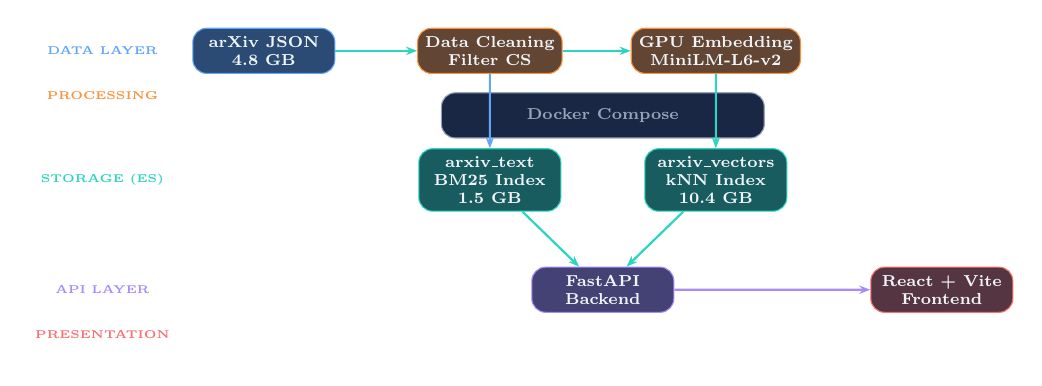
\begin{tikzpicture}[
    box/.style={rectangle, rounded corners=5pt, minimum height=0.7cm, align=center, font=\scriptsize\bfseries, minimum width=2.2cm, draw},
    layer/.style={rectangle, rounded corners=3pt, minimum height=0.7cm, font=\tiny\bfseries, text=textMuted, draw=none},
    arr/.style={-{Stealth[length=4pt]}, thick, accentTeal},
    scale=0.82, transform shape
]
% Data Layer
\node[box, fill=accentBlue!35!primaryDark, draw=accentBlue, text=textWhite] (raw) at (0,0) {arXiv JSON\\4.8 GB};
\node[layer] at (-2.5,0) {\textcolor{accentBlue}{DATA LAYER}};

% Processing Layer
\node[box, fill=accentOrange!35!primaryDark, draw=accentOrange, text=textWhite] (clean) at (3.5,0) {Data Cleaning\\Filter CS};
\node[box, fill=accentOrange!35!primaryDark, draw=accentOrange, text=textWhite] (embed) at (7,0) {GPU Embedding\\MiniLM-L6-v2};
\node[layer] at (-2.5,-0.7) {\textcolor{accentOrange}{PROCESSING}};

% Storage Layer
\node[box, fill=accentTeal!35!primaryDark, draw=accentTeal, text=textWhite] (bm25idx) at (3.5,-2) {arxiv\_text\\BM25 Index\\1.5 GB};
\node[box, fill=accentTeal!35!primaryDark, draw=accentTeal, text=textWhite] (knnidx) at (7,-2) {arxiv\_vectors\\kNN Index\\10.4 GB};
\node[layer] at (-2.5,-2) {\textcolor{accentTeal}{STORAGE (ES)}};

% API Layer
\node[box, fill=accentPurple!35!primaryDark, draw=accentPurple, text=textWhite] (api) at (5.25,-3.7) {FastAPI\\Backend};
\node[layer] at (-2.5,-3.7) {\textcolor{accentPurple}{API LAYER}};

% UI Layer
\node[box, fill=accentRed!30!primaryDark, draw=accentRed, text=textWhite] (ui) at (10.5,-3.7) {React + Vite\\Frontend};
\node[layer] at (-2.5,-4.4) {\textcolor{accentRed}{PRESENTATION}};

% Docker
\node[box, fill=primaryMid, draw=textMuted, text=textMuted, minimum width=5cm, align=center] (docker) at (5.25,-1) {\textbf{Docker Compose}};

% Arrows
\draw[arr] (raw) -- (clean);
\draw[arr] (clean) -- (embed);
\draw[arr] (embed) -- (knnidx);
\draw[arr, accentBlue] (clean) -- (bm25idx);
\draw[arr] (bm25idx) -- (api);
\draw[arr] (knnidx) -- (api);
\draw[arr, accentPurple] (api) -- (ui);

\end{tikzpicture}
\end{center}

\vspace{0.05cm}
{\footnotesize
\textbf{Công nghệ}: Python 3.x, Elasticsearch 8.12, Docker, FastAPI, React + Vite, Kibana\\
\textbf{Kiến trúc Dual-Index}: Tách Keyword Search (BM25 Index) và Semantic Search (kNN Index) để tối ưu hóa lưu trữ và truy vấn}
\end{frame}

% ── SLIDE 14: Data Ingestion Flow ──
\begin{frame}{Data Ingestion Flow}
\begin{center}
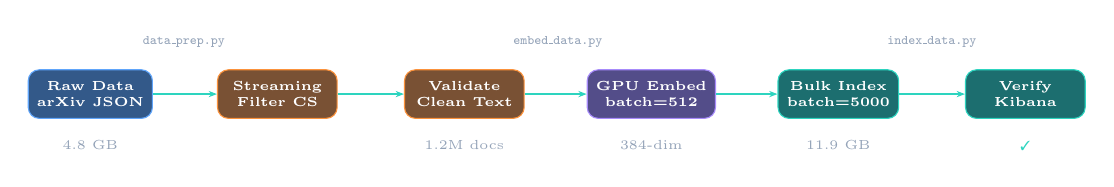
\begin{tikzpicture}[
    stepbox/.style={rectangle, rounded corners=4pt, minimum height=0.65cm, align=center, font=\tiny\bfseries, minimum width=1.6cm, draw, text=white},
    arr/.style={-{Stealth[length=3pt]}, thick, accentTeal},
    lbl/.style={font=\tiny\color{textMuted}, above},
    scale=0.95, transform shape
]
% Steps
\node[stepbox, fill=accentBlue!45!primaryDark, draw=accentBlue] (s1) at (0,0) {Raw Data\\arXiv JSON};
\node[stepbox, fill=accentOrange!45!primaryDark, draw=accentOrange] (s2) at (2.5,0) {Streaming\\Filter CS};
\node[stepbox, fill=accentOrange!45!primaryDark, draw=accentOrange] (s3) at (5,0) {Validate\\Clean Text};
\node[stepbox, fill=accentPurple!45!primaryDark, draw=accentPurple] (s4) at (7.5,0) {GPU Embed\\batch=512};
\node[stepbox, fill=accentTeal!45!primaryDark, draw=accentTeal] (s5) at (10,0) {Bulk Index\\batch=5000};
\node[stepbox, fill=accentTeal!45!primaryDark, draw=accentTeal] (s6) at (12.5,0) {Verify\\Kibana};

% Arrows
\draw[arr] (s1) -- (s2);
\draw[arr] (s2) -- (s3);
\draw[arr] (s3) -- (s4);
\draw[arr] (s4) -- (s5);
\draw[arr] (s5) -- (s6);

% Labels
\node[lbl] at (1.25,0.5) {\texttt{data\_prep.py}};
\node[lbl] at (6.25,0.5) {\texttt{embed\_data.py}};
\node[lbl] at (11.25,0.5) {\texttt{index\_data.py}};

% Data sizes
\node[font=\tiny\color{textMuted}, below] at (0,-0.5) {4.8 GB};
\node[font=\tiny\color{textMuted}, below] at (5,-0.5) {1.2M docs};
\node[font=\tiny\color{textMuted}, below] at (7.5,-0.5) {384-dim};
\node[font=\tiny\color{textMuted}, below] at (10,-0.5) {11.9 GB};
\node[font=\tiny\color{accentTeal}, below] at (12.5,-0.5) {\cmark};

\end{tikzpicture}
\end{center}

\vspace{0.3cm}

\begin{columns}[T]
\begin{column}{0.48\textwidth}
\begin{block}{Các bước chính}
{\small
\begin{enumerate}
    \item \textbf{Streaming}: Đọc line-by-line (tránh OOM 4.8GB)
    \item \textbf{Filter}: Lọc category \texttt{cs.*} $\to$ 1.2M
    \item \textbf{Clean}: Chuẩn hóa text, trích năm
\end{enumerate}
}
\end{block}
\end{column}
\begin{column}{0.48\textwidth}
\begin{block}{Giai đoạn 2}
{\small
\begin{enumerate}\setcounter{enumi}{3}
    \item \textbf{GPU Embed}: Tesla T4, batch 512
    \item \textbf{Bulk Index}: ES \texttt{helpers.bulk()}, 5000/batch
    \item \textbf{Verify}: Kibana kiểm tra count/mapping
\end{enumerate}
}
\end{block}
\end{column}
\end{columns}
\end{frame}

% ── SLIDE 15: Search Flow ──
\begin{frame}{Search Flow --- Hybrid Search Pipeline}
\begin{center}
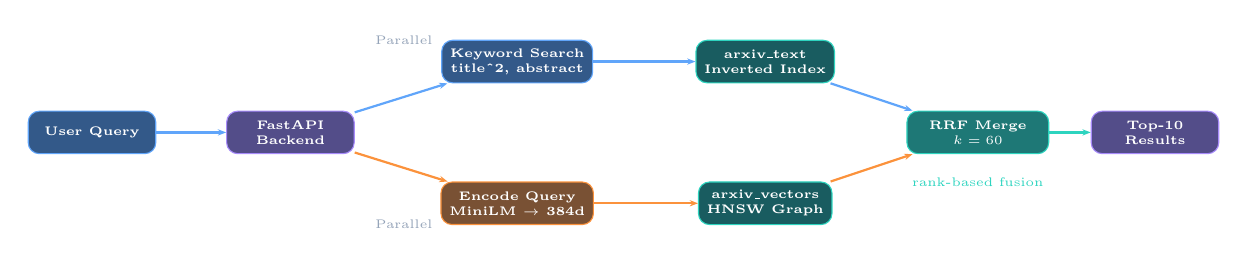
\begin{tikzpicture}[
    box/.style={rectangle, rounded corners=4pt, minimum height=0.6cm, align=center, font=\tiny\bfseries, minimum width=1.8cm, draw, text=white},
    arr/.style={-{Stealth[length=3pt]}, thick},
    scale=0.9, transform shape
]
% User Query
\node[box, fill=accentBlue!45!primaryDark, draw=accentBlue] (q) at (0,0) {User Query};
\node[box, fill=accentPurple!45!primaryDark, draw=accentPurple] (api) at (2.8,0) {FastAPI\\Backend};

% Branch
\node[box, fill=accentBlue!45!primaryDark, draw=accentBlue] (bm25) at (6, 1) {Keyword Search\\title\^{}2, abstract};
\node[box, fill=accentOrange!45!primaryDark, draw=accentOrange] (enc) at (6, -1) {Encode Query\\MiniLM $\to$ 384d};

% Indices
\node[box, fill=accentTeal!35!primaryDark, draw=accentTeal] (idx1) at (9.5, 1) {arxiv\_text\\Inverted Index};
\node[box, fill=accentTeal!35!primaryDark, draw=accentTeal] (idx2) at (9.5, -1) {arxiv\_vectors\\HNSW Graph};

% Merge
\node[box, fill=accentTeal!50!primaryDark, draw=accentTeal, minimum width=2cm] (rrf) at (12.5, 0) {RRF Merge\\$k=60$};

% Results
\node[box, fill=accentPurple!45!primaryDark, draw=accentPurple] (res) at (15, 0) {Top-10\\Results};

% Arrows
\draw[arr, accentBlue] (q) -- (api);
\draw[arr, accentBlue] (api) -- (bm25);
\draw[arr, accentOrange] (api) -- (enc);
\draw[arr, accentBlue] (bm25) -- (idx1);
\draw[arr, accentOrange] (enc) -- (idx2);
\draw[arr, accentBlue] (idx1) -- (rrf);
\draw[arr, accentOrange] (idx2) -- (rrf);
\draw[arr, accentTeal] (rrf) -- (res);

% Labels
\node[font=\tiny\color{textMuted}] at (4.4, 1.3) {Parallel};
\node[font=\tiny\color{textMuted}] at (4.4, -1.3) {Parallel};
\node[font=\tiny\color{accentTeal}] at (12.5, -0.7) {rank-based fusion};

\end{tikzpicture}
\end{center}

\vspace{0.2cm}

\begin{columns}[T]
\begin{column}{0.32\textwidth}
\begin{block}{\small\textcolor{accentBlue}{Keyword Stream}}
{\scriptsize
\texttt{multi\_match} trên \texttt{title\^{}2, abstract}\\
$\to$ Top 30 kết quả\\
$\to$ \textbf{Inverted Index} ($O(1)$)
}
\end{block}
\end{column}
\begin{column}{0.32\textwidth}
\begin{block}{\small\textcolor{accentOrange}{Semantic Stream}}
{\scriptsize
Encode query $\to$ 384d vector\\
$\to$ Cosine similarity, $k=10$\\
$\to$ \textbf{HNSW graph} ($O(\log N)$)
}
\end{block}
\end{column}
\begin{column}{0.32\textwidth}
\begin{exampleblock}{\small\textcolor{accentTeal}{RRF Merge}}
{\scriptsize
Gộp theo \textbf{thứ hạng}\\
$\to$ $\frac{1}{k+rank}$ mỗi stream\\
$\to$ Sort $\to$ \textbf{Top 10}
}
\end{exampleblock}
\end{column}
\end{columns}
\end{frame}
    % System Architecture, Data Flow, Search Flow
% ============================================================
% CHƯƠNG 6: Embedding Pipeline — Model Selection, GPU, Checkpoint
% ============================================================
\section{Embedding Pipeline}

% ── SLIDE 16: Model Selection ──
\begin{frame}{Lựa chọn Embedding Model}
\centering
\renewcommand{\arraystretch}{1.05}
{\small
\begin{tabular}{l c c c l}
\toprule
\textbf{Model} & \textbf{Dims} & \textbf{MTEB} & \textbf{Params} & \textbf{Ghi chú} \\
\midrule
\rowcolor{highlightRow}
\textcolor{accentTeal}{\textbf{all-MiniLM-L6-v2}} & \textcolor{accentTeal}{\textbf{384}} & \textcolor{accentTeal}{\textbf{56}} & \textcolor{accentTeal}{\textbf{22M}} & \textcolor{accentTeal}{\textbf{Nhanh, nhẹ, cân bằng}} \\
bge-small-en-v1.5 & 384 & 62 & 33M & BAAI, chất lượng cao \\
e5-large-v2 & 1024 & 64 & 335M & Microsoft, nặng \\
SPECTER2 & 768 & --- & 110M & Chuyên academic \\
\bottomrule
\end{tabular}
}

\vspace{0.1cm}

\begin{columns}[T]
\begin{column}{0.48\textwidth}
\begin{exampleblock}{Lý do chọn MiniLM-L6-v2}
{\footnotesize
\begin{itemize}\itemsep0pt \parskip0pt \parsep0pt
    \item \textbf{384 dims}: Tiết kiệm RAM \& storage
    \item \textbf{22M params}: Chạy được trên Colab free
    \item \textbf{14K+ sentences/sec} (GPU)
    \item Cân bằng tốt giữa chất lượng và tốc độ
\end{itemize}
}
\end{exampleblock}
\end{column}
\begin{column}{0.48\textwidth}
\begin{block}{Đầu vào model}
{\footnotesize
$T_{\text{input}} = \text{Title} \;\|\; \text{[SEP]} \;\|\; \text{Abstract}$

\vspace{0.05cm}
\begin{itemize}\itemsep0pt \parskip0pt \parsep0pt
    \item Token limit: 256 tokens
    \item Title: $\sim$15 tokens
    \item Abstract budget: 240 tokens $\approx$ 960 chars
    \item Cắt theo ranh giới câu (smart truncation)
\end{itemize}
}
\end{block}
\end{column}
\end{columns}
\end{frame}

% ── SLIDE 17: GPU Pipeline ──
\begin{frame}{GPU Acceleration và Batch Processing}
\begin{columns}[T]
\begin{column}{0.48\textwidth}

\begin{alertblock}{Vấn đề: CPU quá chậm}
{\footnotesize
\begin{itemize}\itemsep0pt \parskip0pt \parsep0pt
    \item CPU: \textbf{5-10 docs/sec}
    \item 1.2M docs $\to$ \textbf{33-66 giờ!}
    \item Không khả thi cho Big Data
\end{itemize}
}
\end{alertblock}

\vspace{0.05cm}

\begin{exampleblock}{Giải pháp: Google Colab + GPU}
{\footnotesize
\begin{itemize}\itemsep0pt \parskip0pt \parsep0pt
    \item \textbf{Tesla T4} (16GB VRAM)
    \item \textbf{500-800 docs/sec} ($\sim$80x nhanh hơn)
    \item Batch size: \textbf{512}
    \item Dynamic padding (tiết kiệm VRAM)
\end{itemize}
}
\end{exampleblock}

\end{column}
\begin{column}{0.48\textwidth}

\begin{block}{Kỹ thuật tối ưu}
{\footnotesize
\begin{enumerate}\itemsep0pt \parskip0pt \parsep0pt
    \item \textbf{Batch Processing}: 512 docs/batch, encode song song
    \item \textbf{Dynamic Padding}: Pad theo batch dài nhất
    \item \textbf{Smart Truncation}: Giữ ranh giới câu $\leq$ 960 chars
    \item \textbf{tqdm Progress}: Theo dõi tiến trình real-time
\end{enumerate}
}
\end{block}

\vspace{0.05cm}

\centering
\renewcommand{\arraystretch}{0.95}
{\footnotesize
\begin{tabular}{l r}
\toprule
\textbf{Chỉ số} & \textbf{Giá trị} \\
\midrule
Tổng tài liệu & 1,203,108 \\
Thời gian & \textcolor{accentTeal}{\textbf{$\sim$35 phút}} \\
Output & 11.05 GB JSONL \\
\bottomrule
\end{tabular}
}

\end{column}
\end{columns}
\end{frame}

% ── SLIDE 18: Checkpoint ──
\begin{frame}{Checkpoint \& Resume + Kết quả}
\begin{columns}[T]
\begin{column}{0.48\textwidth}

\begin{block}{Cơ chế Checkpoint}
{\footnotesize
\begin{itemize}\itemsep0pt \parskip0pt \parsep0pt
    \item Lưu \texttt{progress.json} mỗi \textbf{50,000 docs}
    \item Backup lên \textbf{Google Drive} (Colab)
    \item Tự động resume khi bị disconnect
    \item Không mất dữ liệu đã xử lý
\end{itemize}
}
\end{block}

\vspace{0.05cm}

\begin{exampleblock}{Tại sao cần Checkpoint?}
{\footnotesize
\begin{itemize}\itemsep0pt \parskip0pt \parsep0pt
    \item Google Colab có \textbf{timeout} (12h free)
    \item Network disconnect bất kỳ lúc nào
    \item 1.2M docs = nhiều batch $\to$ cần fault tolerance
\end{itemize}
}
\end{exampleblock}

\end{column}
\begin{column}{0.48\textwidth}

\begin{block}{Tổng kết Embedding Pipeline}
\centering
\renewcommand{\arraystretch}{1.0}
{\footnotesize
\begin{tabular}{l r}
\toprule
\textbf{Chỉ số} & \textbf{Giá trị} \\
\midrule
Model & MiniLM-L6-v2 \\
Dimensions & 384 \\
Parameters & 22M \\
Hardware & Tesla T4 (16GB) \\
Batch size & 512 \\
Tốc độ & 500-800 docs/sec \\
Tổng tài liệu & 1,203,108 \\
Thời gian & \textbf{$\sim$35 phút} \\
Output file & 11.05 GB \\
Checkpoint & /50K docs \\
\bottomrule
\end{tabular}
}
\end{block}

\end{column}
\end{columns}
\end{frame}
       % Model Selection, GPU Pipeline, Checkpoint
% ============================================================
% CHƯƠNG 7: Search Implementation — Keyword, Semantic, Hybrid
% ============================================================
\section{Search Implementation}

% ── SLIDE 19: Keyword Search ──
\begin{frame}[fragile]{Keyword Search --- Keyword Matching}
\begin{columns}[T]
\begin{column}{0.48\textwidth}

\begin{block}{Query DSL}
\begin{lstlisting}[language=Python]
{
  "query": {
    "multi_match": {
      "query": "<user_query>",
      "fields": ["title^2",
                 "abstract"],
      "type": "best_fields"
    }
  },
  "size": 10
}
\end{lstlisting}
\end{block}

\end{column}
\begin{column}{0.48\textwidth}

\begin{block}{Giải thích}
{\scriptsize
\begin{itemize}\itemsep0pt \parskip0pt \parsep0pt
    \item \textbf{multi\_match}: Tìm trên nhiều field
    \item \textbf{title\^{}2}: Boost title gấp 2 lần
    \item \textbf{best\_fields}: Score theo field match tốt nhất
    \item \textbf{Index}: \texttt{arxiv\_text} (1.5 GB)
\end{itemize}
}
\end{block}

\vspace{0.1cm}

\begin{exampleblock}{Ưu điểm}
{\scriptsize
\begin{itemize}\itemsep0pt \parskip0pt \parsep0pt
    \item Nhanh: $\sim$70ms P50 ở 1.2M
    \item Chính xác cho thuật ngữ, tên riêng
    \item Nhẹ tài nguyên (text only)
\end{itemize}
}
\end{exampleblock}

\end{column}
\end{columns}
\end{frame}

% ── SLIDE 20: Semantic Search ──
\begin{frame}[fragile]{Semantic Search --- Semantic Understanding}
\begin{columns}[T]
\begin{column}{0.48\textwidth}

\begin{block}{Query DSL}
\begin{lstlisting}[language=Python]
{
  "knn": {
    "field": "embedding",
    "query_vector": [0.12, ...],
    "k": 10, "num_candidates": 100
  }
}
\end{lstlisting}
\end{block}

\vspace{-0.1cm}

\begin{block}{Pipeline}
{\scriptsize
\begin{enumerate}\itemsep0pt \parskip0pt \parsep0pt
    \item Encode query $\to$ 384-dim vector
    \item HNSW graph traversal
    \item Cosine similarity ranking
    \item Trả về top-$k$ nearest neighbors
\end{enumerate}
}
\end{block}

\end{column}
\begin{column}{0.48\textwidth}

\begin{block}{Giải thích}
{\scriptsize
\begin{itemize}\itemsep0pt \parskip0pt \parsep0pt
    \item \textbf{field}: \texttt{embedding} (384-dim vector)
    \item \textbf{k=10}: Trả về 10 kết quả gần nhất
    \item \textbf{num\_candidates=100}: Duyệt 100 ứng viên/shard
    \item \textbf{Index}: \texttt{arxiv\_vectors} (10.4 GB)
\end{itemize}
}
\end{block}

\vspace{-0.1cm}

\begin{exampleblock}{Ưu điểm}
{\scriptsize
\begin{itemize}\itemsep0pt \parskip0pt \parsep0pt
    \item Hiểu từ đồng nghĩa, paraphrase tốt
    \item Tìm kiếm trực tiếp bằng câu tự nhiên
    \item VD: ``detect fake images'' $\approx$ ``deepfake''
\end{itemize}
}
\end{exampleblock}

\end{column}
\end{columns}
\end{frame}

% ── SLIDE 21: Hybrid Search ──
\begin{frame}{Hybrid Search --- Kết hợp tất cả}
\begin{columns}[T]
\begin{column}{0.46\textwidth}

\begin{block}{Cách hoạt động}
{\scriptsize
\begin{enumerate}\itemsep0pt \parskip0pt \parsep0pt
    \item \textbf{Parallel queries}:\\
    Keyword $\to$ \texttt{arxiv\_text} (top 30)\\
    Semantic $\to$ \texttt{arxiv\_vectors} (top 30)
    \item \textbf{Extract} document IDs từ cả hai
    \item \textbf{Compute RRF score}:\\
    $RRF(d) = \sum \frac{1}{60 + rank(d)}$
    \item \textbf{Sort} theo RRF score giảm dần
    \item \textbf{Return} top 10
    \item \textbf{Enrich} metadata qua \texttt{es.mget()}
\end{enumerate}
}
\end{block}

\end{column}
\begin{column}{0.50\textwidth}

\begin{exampleblock}{Kiến trúc Dual-Index}
{\scriptsize
\begin{itemize}\itemsep0pt \parskip0pt \parsep0pt
    \item \textbf{arxiv\_text} (1.5 GB): Chỉ từ khóa $\to$ nhanh, nhẹ
    \item \textbf{arxiv\_vectors} (10.4 GB): Vector 384d $\to$ ngữ nghĩa qua HNSW
    \item Tách riêng $\to$ tối ưu lưu trữ và query độc lập
    \item Incremental ingestion: thêm bài báo mới qua API
\end{itemize}
}
\end{exampleblock}

\vspace{-0.1cm}

\begin{block}{Tối ưu ES Indexing}
{\scriptsize
\begin{itemize}\itemsep0pt \parskip0pt \parsep0pt
    \item 2 shards (giảm từ 5 để khớp số node thực)
    \item 0 replicas (single node cho dev env)
    \item \texttt{refresh\_interval=-1} khi bulk load
    \item \texttt{\_forcemerge} sau bulk để tối ưu HNSW
    \item JVM Heap: 4GB
\end{itemize}
}
\end{block}

\end{column}
\end{columns}
\end{frame}
          % BM25 Search, kNN Search, Hybrid RRF
% ============================================================
% CHƯƠNG 8: Evaluation — Methodology, Metrics, Results, Analysis
% ============================================================
\section{Đánh giá chất lượng}

% ── SLIDE 22: Methodology ──
\begin{frame}{Phương pháp đánh giá}
\begin{columns}[T]
\begin{column}{0.48\textwidth}

\begin{block}{Ground Truth Construction}
{\small
\begin{itemize}
    \item \textbf{30 test queries}, chia 3 nhóm (10 mỗi nhóm):
\end{itemize}
}

\vspace{0.05cm}

{\scriptsize
\begin{tabular}{l l}
\toprule
\textbf{Nhóm} & \textbf{Ví dụ query} \\
\midrule
\textcolor{accentBlue}{\textbf{A. Exact}} & ``BERT fine-tuning'' \\
\textcolor{accentOrange}{\textbf{B. Semantic}} & ``methods to detect fake images'' \\
\textcolor{accentTeal}{\textbf{C. Mixed}} & ``transformer for NLP tasks'' \\
\bottomrule
\end{tabular}
}
\end{block}

\end{column}
\begin{column}{0.48\textwidth}

\begin{block}{Quy trình gán nhãn}
{\small
\begin{enumerate}
    \item \textbf{Pooling}: Top 10 từ mỗi method $\to$ merge $\to$ 15-25 candidates/query
    \item \textbf{Silver Standard}: Majority voting\\
    Relevant (1) nếu xuất hiện $\geq 2/3$ methods\\
    Irrelevant (0) nếu chỉ 1 method
    \item \textbf{Manual verification} trên tập con
\end{enumerate}
}
\end{block}

\vspace{0.1cm}

{\footnotesize \textbf{Tổng}: 30 queries $\times$ $\sim$20 candidates $=$ $\sim$600 judgments}

\end{column}
\end{columns}
\end{frame}

% ── SLIDE 23: Metrics ──
\begin{frame}{Metrics: NDCG@10 và MRR@10}
\begin{columns}[T]
\begin{column}{0.48\textwidth}

\begin{block}{NDCG@10 {\scriptsize (Normalized DCG)}}
{\footnotesize
\textbf{DCG@p}: Đánh giá chất lượng xếp hạng
\[
DCG@p = \sum_{i=1}^{p} \frac{2^{rel_i} - 1}{\log_2(i+1)}
\]

\textbf{NDCG@p}: Chuẩn hóa về [0,1]
\[
NDCG@p = \frac{DCG@p}{IDCG@p}
\]

\begin{itemize}\itemsep0pt \parskip0pt \parsep0pt
    \item IDCG = DCG của \textit{perfect ranking}
    \item Vị trí đầu quan trọng hơn
    \item \textbf{1.0 = hoàn hảo}
\end{itemize}
}
\end{block}

\end{column}
\begin{column}{0.48\textwidth}

\begin{block}{MRR@10 {\scriptsize (Mean Reciprocal Rank)}}
{\footnotesize
\[
RR = \frac{1}{rank^*}
\]

\begin{itemize}\itemsep0pt \parskip0pt \parsep0pt
    \item $rank^*$ = vị trí tài liệu relevant \textbf{đầu tiên}
    \item Nếu không có trong top 10: $RR = 0$
    \item MRR = trung bình RR trên tất cả queries
    \item \textbf{1.0 = luôn đúng ở vị trí 1}
\end{itemize}
}
\end{block}

\vspace{0.05cm}

\begin{exampleblock}{Tại sao chọn 2 metrics?}
{\footnotesize
\begin{itemize}\itemsep0pt \parskip0pt \parsep0pt
    \item \textbf{NDCG}: Đánh giá \textit{toàn bộ} top 10
    \item \textbf{MRR}: Đánh giá \textit{kết quả đầu tiên}
\end{itemize}
}
\end{exampleblock}

\end{column}
\end{columns}
\end{frame}

% ── SLIDE 24: Results Overview - Table ──
\begin{frame}{Kết quả đánh giá --- Bảng tổng quan}
\centering
\renewcommand{\arraystretch}{1.1}
{\small
\begin{tabular}{l c c c c c c}
\toprule
\multirow{2}{*}{\textbf{Phương pháp}} & \multicolumn{2}{c}{\textbf{Group A (Exact)}} & \multicolumn{2}{c}{\textbf{Group B (Semantic)}} & \multicolumn{2}{c}{\textbf{Group C (Mixed)}} \\
\cmidrule(lr){2-3} \cmidrule(lr){4-5} \cmidrule(lr){6-7}
& NDCG & MRR & NDCG & MRR & NDCG & MRR \\
\midrule
Keyword (BM25) & 0.6407 & 0.8750 & 0.6780 & 1.0000 & 0.6967 & 1.0000 \\
Semantic (kNN) & 0.6554 & 0.9250 & 0.6632 & 1.0000 & 0.6774 & 1.0000 \\
\rowcolor{highlightRow}
\textcolor{accentTeal}{\textbf{Hybrid (RRF)}} & \textcolor{accentTeal}{\textbf{0.9752}} & \textcolor{accentTeal}{\textbf{1.0000}} & \textcolor{accentTeal}{\textbf{0.9469}} & \textcolor{accentTeal}{0.9250} & \textcolor{accentTeal}{\textbf{0.9821}} & \textcolor{accentTeal}{\textbf{1.0000}} \\
\bottomrule
\end{tabular}
}

\vspace{0.05cm}

\begin{block}{Nhận xét tổng quan}
{\footnotesize
\begin{itemize}\itemsep0pt \parskip0pt \parsep0pt
    \item \textbf{Keyword (BM25)} và \textbf{Semantic (kNN)} đơn lẻ đạt hiệu năng khá tốt ($\sim$0.64 - 0.70 NDCG).
    \item \textbf{Hybrid (RRF)} cải thiện vượt trội lên mức \textbf{0.94 - 0.98 NDCG} nhờ bù trừ điểm yếu của nhau.
\end{itemize}
}
\end{block}
\end{frame}

% ── SLIDE 25: Results Overview - Charts ──
\begin{frame}{Kết quả đánh giá --- Biểu đồ so sánh}
\begin{columns}[T]
\begin{column}{0.48\textwidth}
\begin{center}
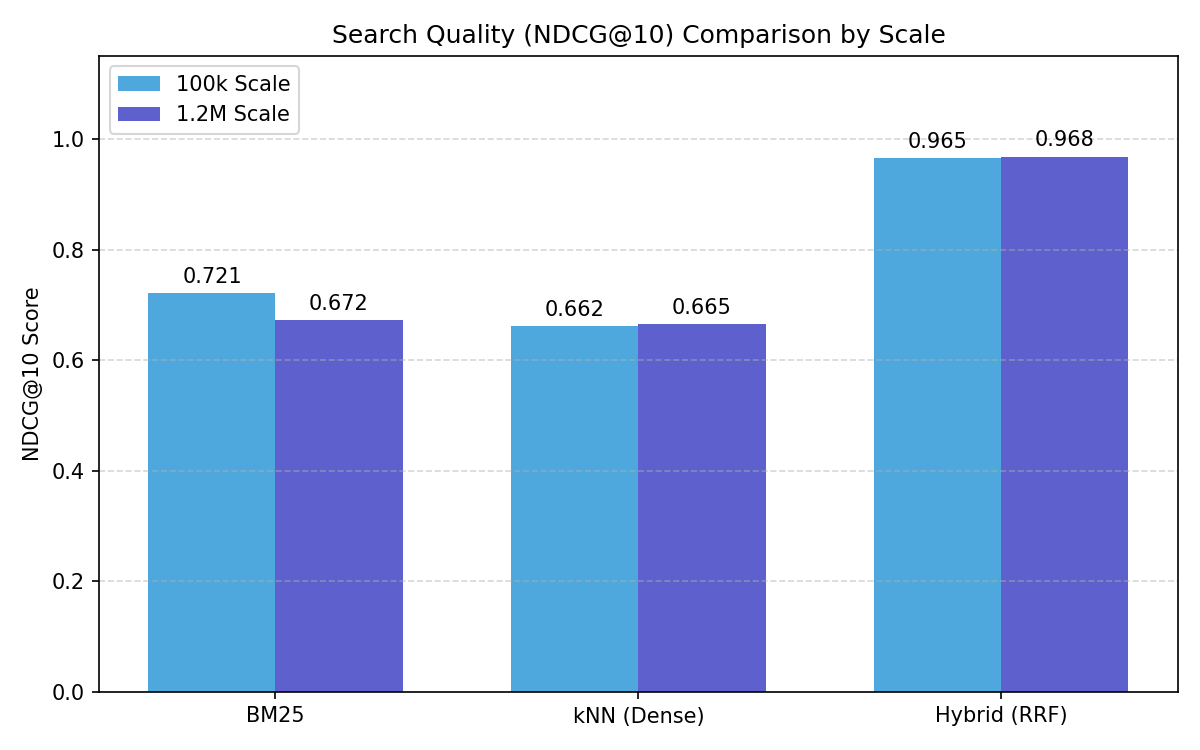
\includegraphics[width=\textwidth]{ndcg_comparison.png}

\vspace{0.1cm}
{\scriptsize So sánh NDCG@10 giữa các phương thức}
\end{center}
\end{column}
\begin{column}{0.48\textwidth}
\begin{center}
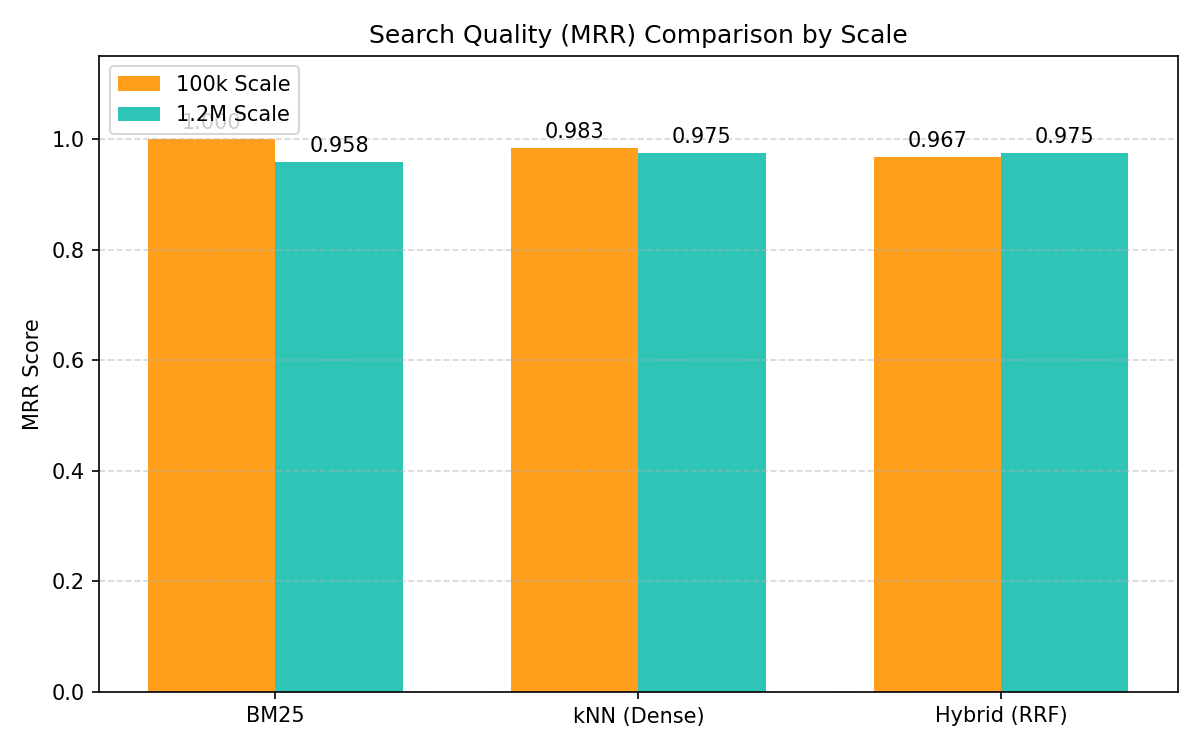
\includegraphics[width=\textwidth]{mrr_comparison.png}

\vspace{0.1cm}
{\scriptsize So sánh MRR@10 giữa các phương thức}
\end{center}
\end{column}
\end{columns}
\end{frame}

% ── SLIDE 26: Analysis ──
\begin{frame}{Phân tích chi tiết}
\begin{columns}[T]
\begin{column}{0.48\textwidth}

\begin{block}{Overlap Analysis}
{\footnotesize
Trung bình chỉ \textbf{1.5/10} docs trùng lặp giữa Keyword và Semantic

\vspace{0.05cm}
$\Rightarrow$ Hai phương pháp tìm kết quả \textbf{rất khác nhau}\\
$\Rightarrow$ Hybrid kết hợp cả hai $\to$ NDCG tăng từ $\sim$0.67 lên $\sim$0.97
}
\end{block}

\vspace{0.05cm}

\begin{exampleblock}{Tại sao Hybrid vượt trội?}
{\scriptsize
\begin{itemize}\itemsep0pt \parskip0pt \parsep0pt
    \item Keyword search tìm đúng \textbf{thuật ngữ chính xác}
    \item Semantic search tìm đúng \textbf{ý nghĩa tương đồng}
    \item RRF promote docs được \textbf{cả hai đồng ý}
    \item Docs chỉ 1 method $\to$ rank thấp hơn
\end{itemize}
}
\end{exampleblock}

\end{column}
\begin{column}{0.48\textwidth}

\begin{block}{Scale Stability (100K $\to$ 1.2M)}
\centering
\renewcommand{\arraystretch}{1.0}
{\scriptsize
\begin{tabular}{l c c}
\toprule
\textbf{Phương pháp} & \textbf{100K} & \textbf{1.2M} \\
\midrule
Keyword (BM25) & 0.7212 & 0.6718 {\scriptsize\textcolor{accentRed}{$\downarrow$}} \\
Semantic (kNN) & 0.6676 & 0.6653 {\scriptsize\textcolor{textMuted}{$\approx$}} \\
\rowcolor{highlightRow}
\textcolor{accentTeal}{Hybrid (RRF)} & \textcolor{accentTeal}{0.9626} & \textcolor{accentTeal}{0.9681} {\scriptsize\textcolor{accentTeal}{$\approx$}} \\
\bottomrule
\end{tabular}
}
\end{block}

\vspace{0.05cm}

\begin{alertblock}{Key Insights}
{\scriptsize
\begin{itemize}\itemsep0pt \parskip0pt \parsep0pt
    \item Keyword search \textbf{giảm nhẹ} khi scale (noise tăng)
    \item Semantic search \textbf{ổn định} (vector space bền vững)
    \item Hybrid \textbf{ổn định nhất}: NDCG $\sim$0.96-0.97 ở mọi scale
\end{itemize}
}
\end{alertblock}

\end{column}
\end{columns}
\end{frame}
      % Methodology, Metrics, Results, Analysis
% ============================================================
% CHƯƠNG 9: Benchmarking — Latency, Scaling, Storage
% ============================================================
\section{Đánh giá hiệu năng}

% ── SLIDE 27: Latency Analysis - Table ──
\begin{frame}{Latency Analysis --- Bảng tổng quan}
\centering
\renewcommand{\arraystretch}{1.1}
{\small
\begin{tabular}{l *{6}{c}}
\toprule
\multirow{2}{*}{\textbf{Phương pháp}} & \multicolumn{2}{c}{\textbf{100K}} & \multicolumn{2}{c}{\textbf{500K}} & \multicolumn{2}{c}{\textbf{1.2M}} \\
\cmidrule(lr){2-3} \cmidrule(lr){4-5} \cmidrule(lr){6-7}
& P50 & P95 & P50 & P95 & P50 & P95 \\
\midrule
Keyword (BM25) & 15 & 56 & 21 & 37 & 71 & 153 \\
Semantic (kNN) & 13 & 34 & 20 & 41 & 191 & 1206 \\
\rowcolor{highlightRow}
\textcolor{accentTeal}{\textbf{Hybrid (RRF)}} & \textcolor{accentTeal}{30} & \textcolor{accentTeal}{53} & \textcolor{accentTeal}{42} & \textcolor{accentTeal}{62} & \textcolor{accentTeal}{\textbf{99}} & \textcolor{accentTeal}{156} \\
\bottomrule
\end{tabular}
}

\vspace{0.05cm}
{\scriptsize (Đơn vị: milliseconds)}

\vspace{0.15cm}

\begin{exampleblock}{Nhận xét về độ trễ}
{\small
\begin{itemize}\itemsep0pt \parskip0pt \parsep0pt
    \item \textbf{Keyword search} duy trì độ trễ rất thấp ở mọi quy mô ($\leq$ 71ms P50).
    \item \textbf{Hybrid Search} đạt hiệu năng ấn tượng với \textbf{99ms P50} ở quy mô 1.2M tài liệu, đáp ứng tốt tiêu chuẩn thời gian thực ($<$ 100ms).
\end{itemize}
}
\end{exampleblock}
\end{frame}

% ── SLIDE 28: Latency Analysis - Charts & Cold Start ──
\begin{frame}{Latency Analysis --- Trực quan hóa \& Thách thức}
\begin{columns}[T]
\begin{column}{0.48\textwidth}
\begin{center}
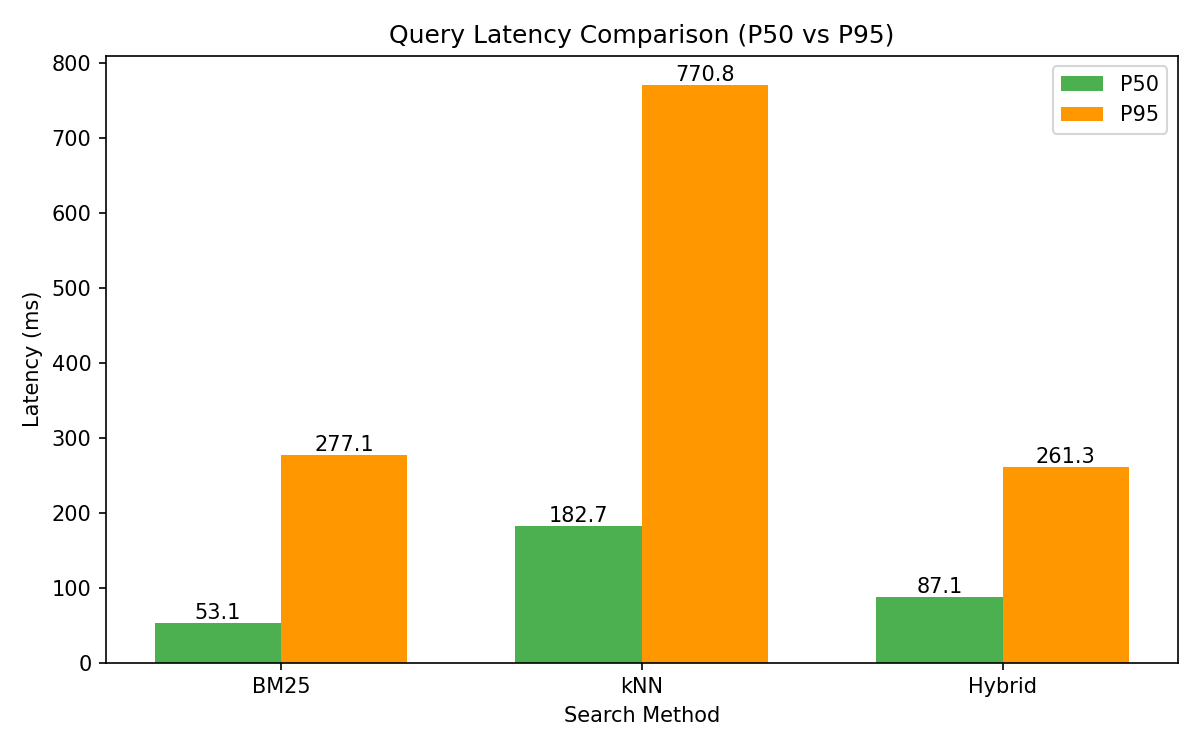
\includegraphics[width=\textwidth]{latency_comparison.png}

\vspace{0.1cm}
{\scriptsize Độ trễ các phương thức ở quy mô 1.2M}
\end{center}
\end{column}
\begin{column}{0.48\textwidth}

\begin{alertblock}{Thách thức: Semantic Cold Start}
{\small
P95 của Semantic đạt \textbf{1,206ms} ở quy mô 1.2M!\\
\textbf{Nguyên nhân}: HNSW graph (10.4GB) dung lượng lớn phải load từ SSD vào Page Cache trong truy vấn đầu tiên.\\
\textbf{Giải pháp}: Cần warmup cache trước khi phục vụ thực tế.
}
\end{alertblock}

\end{column}
\end{columns}
\end{frame}

% ── SLIDE 29: Latency Scaling ──
\begin{frame}{Latency Scaling --- Tăng trưởng theo quy mô}
\begin{columns}[T]
\begin{column}{0.50\textwidth}
\centering
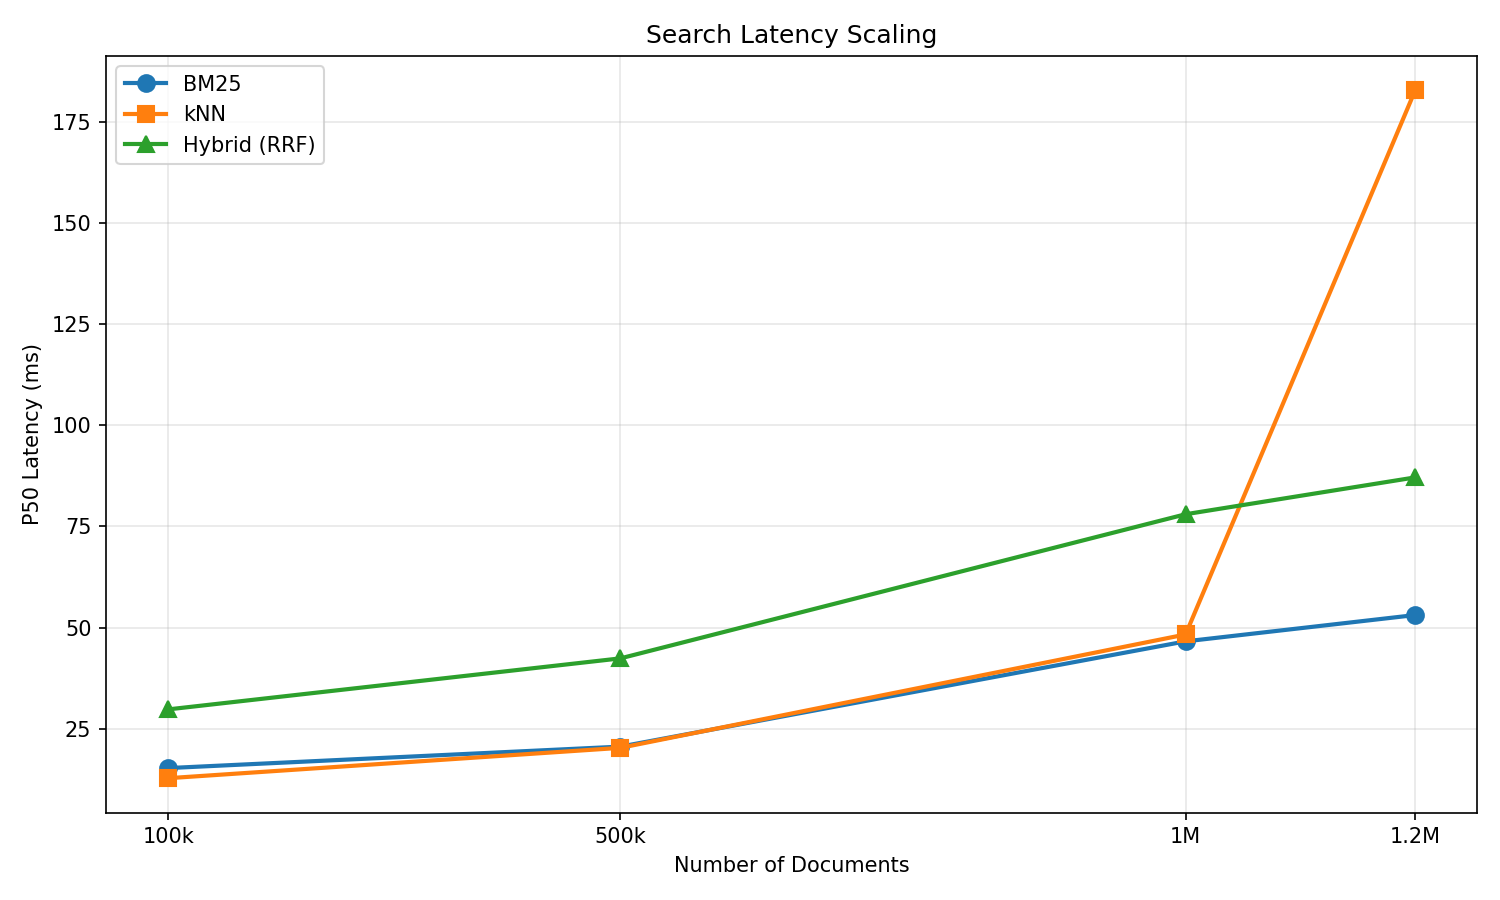
\includegraphics[width=0.95\textwidth]{latency_scaling.png}

\vspace{0.05cm}
{\scriptsize Độ trễ P50 tăng trưởng theo quy mô dữ liệu}
\end{column}
\begin{column}{0.46\textwidth}

\begin{block}{Phân tích Scaling}
{\scriptsize
\begin{itemize}\itemsep0pt \parskip0pt \parsep0pt
    \item \textbf{Keyword}: Inverted Index $O(1)$, tăng tuyến tính chậm khi scale (15ms $\to$ 71ms).
    \item \textbf{Semantic (HNSW)}: Phức tạp $O(\log N)$, tăng nhanh do đồ thị HNSW lớn \& ảnh hưởng IO.
    \item \textbf{Hybrid}: Bị giới hạn bởi stream chậm hơn, nhưng nhờ chạy song song nên tối ưu chỉ còn 99ms P50.
\end{itemize}
}
\end{block}

\vspace{-0.1cm}

\begin{exampleblock}{Môi trường thử nghiệm}
{\scriptsize
\begin{itemize}\itemsep0pt \parskip0pt \parsep0pt
    \item CPU: Intel Core i7-11800H (8 nhân/16 luồng)
    \item RAM: 16GB DDR4 \quad|\quad SSD: NVMe 512GB
    \item ES: Single node trong Docker trên WSL2 Ubuntu
\end{itemize}
}
\end{exampleblock}

\end{column}
\end{columns}
\end{frame}

% ── SLIDE 30: Storage Analysis - Table ──
\begin{frame}{Storage Analysis --- Dung lượng lưu trữ}
\centering
\renewcommand{\arraystretch}{1.1}
{\small
\begin{tabular}{l c c c}
\toprule
\textbf{Quy mô (Docs)} & \textbf{Số tài liệu} & \textbf{Dung lượng JSONL} & \textbf{Dung lượng ES Index} \\
\midrule
100K & 100,000 & 917 MB & 860 MB \\
500K & 500,000 & 4.6 GB & 4.3 GB \\
1.2M & 1,203,108 & 12 GB & 11.9 GB \\
\bottomrule
\end{tabular}
}

\vspace{0.2cm}

\begin{columns}[T]
\begin{column}{0.48\textwidth}
\begin{block}{Phân tích bộ nhớ}
{\footnotesize
\begin{itemize}\itemsep0pt \parskip0pt \parsep0pt
    \item Tăng trưởng dung lượng \textbf{tuyến tính} theo số lượng tài liệu.
    \item Elasticsearch nén tốt hơn raw JSONL nhờ cấu trúc nén khối của Lucene.
\end{itemize}
}
\end{block}
\end{column}
\begin{column}{0.48\textwidth}
\begin{exampleblock}{Dual-Index ở quy mô 1.2M}
{\footnotesize
\begin{tabular}{l r}
\toprule
\textbf{Index} & \textbf{Dung lượng} \\
\midrule
\texttt{arxiv\_text} (BM25) & 1.5 GB \\
\texttt{arxiv\_vectors} (kNN) & 10.4 GB \\
\textbf{Tổng cộng} & \textbf{11.9 GB} \\
\bottomrule
\end{tabular}
}
\end{exampleblock}
\end{column}
\end{columns}
\end{frame}

% ── SLIDE 31: Storage Analysis - Charts ──
\begin{frame}{Storage Analysis --- Trực quan hóa}
\begin{columns}[T]
\begin{column}{0.50\textwidth}
\begin{center}
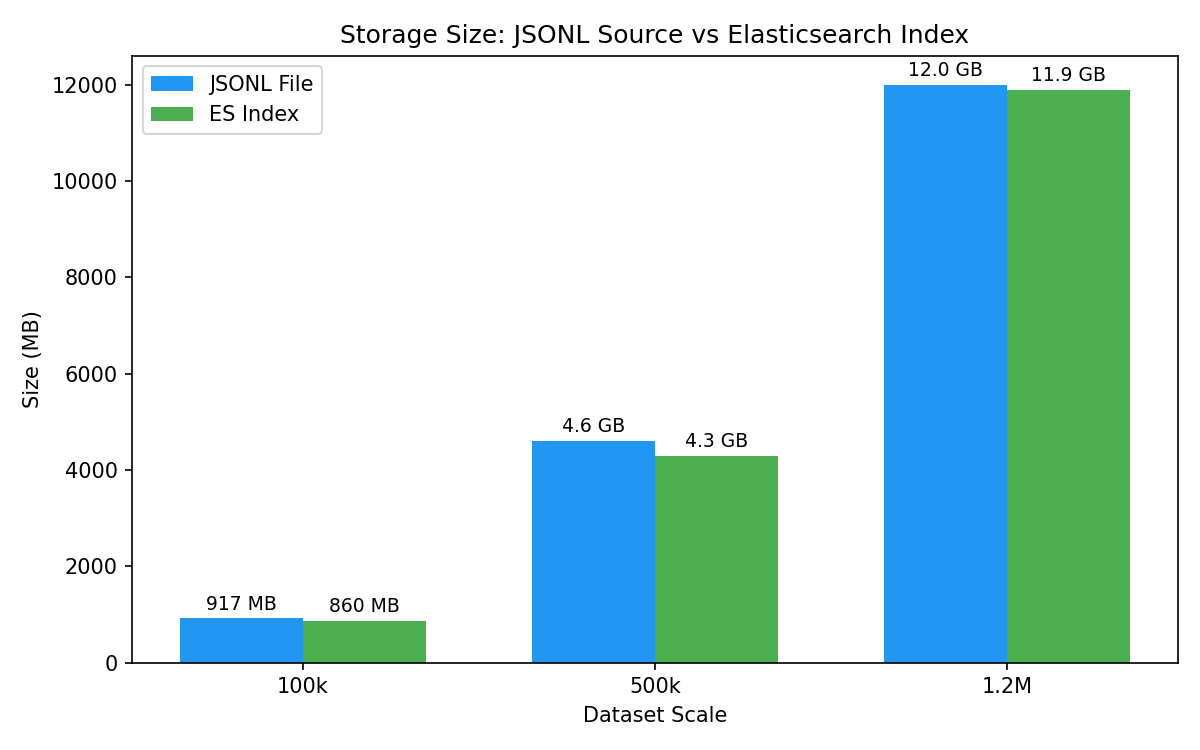
\includegraphics[width=\textwidth]{index_size.png}

\vspace{0.1cm}
{\scriptsize Tăng trưởng dung lượng Index theo quy mô}
\end{center}
\end{column}
\begin{column}{0.46\textwidth}
\begin{block}{Đặc điểm dữ liệu Vector}
{\small
\begin{itemize}\itemsep0pt \parskip0pt \parsep0pt
    \item \textbf{87\%} dung lượng lưu trữ của hệ thống là dành cho \textbf{dữ liệu vector} (HNSW graph).
    \item Mỗi vector nhúng: $384 \text{ dims} \times 4 \text{ bytes} = 1{,}536 \text{ bytes}$.
    \item Việc tách thành Dual-Index giúp truy vấn Keyword search không bị tải dung lượng đồ thị HNSW vào bộ nhớ.
\end{itemize}
}
\end{block}
\end{column}
\end{columns}
\end{frame}
    % Latency, Scaling, Storage
% ============================================================
% CHƯƠNG 11: Kết luận — Tóm tắt, Hạn chế, Demo
% ============================================================
\section{Kết luận}

% ── SLIDE 29: Summary ──
\begin{frame}{Tóm tắt kết quả đạt được}
\begin{enumerate}
    \item[\textcolor{accentTeal}{\cmark}] \textbf{Big Data Pipeline}: Streaming processing 4.8GB, lọc 1.2M bài báo CS không OOM

    \vspace{0.15cm}
    \item[\textcolor{accentTeal}{\cmark}] \textbf{GPU Embedding}: Smart truncation + checkpoint, 1.2M papers embedded trong \textbf{35 phút}

    \vspace{0.15cm}
    \item[\textcolor{accentTeal}{\cmark}] \textbf{Dual-Index Architecture}: \texttt{arxiv\_text} (Keyword) + \texttt{arxiv\_vectors} (Semantic), tối ưu ES indexing

    \vspace{0.15cm}
    \item[\textcolor{accentTeal}{\cmark}] \textbf{Hybrid Search}: NDCG@10 = \textcolor{accentTeal}{\textbf{0.97}}, MRR@10 = \textcolor{accentTeal}{\textbf{0.99}} --- vượt trội Keyword và Semantic search đơn lẻ

    \vspace{0.15cm}
    \item[\textcolor{accentTeal}{\cmark}] \textbf{Comprehensive Evaluation}: 30 queries, 3 nhóm, multi-scale (100K, 500K, 1.2M)

    \vspace{0.15cm}
    \item[\textcolor{accentTeal}{\cmark}] \textbf{Web Application}: FastAPI + React, 3 chế độ search, bộ lọc năm/category, incremental ingestion
\end{enumerate}
\end{frame}

% ── SLIDE 30: Limitations & Future ──
\begin{frame}{Hạn chế và Hướng phát triển}
\begin{columns}[T]
\begin{column}{0.46\textwidth}

\begin{alertblock}{Hạn chế}
{\small
\begin{enumerate}
    \item \textbf{RRF ở application layer}:\\Thêm latency (99ms vs 71ms BM25)
    \item \textbf{Embedding model cơ bản}:\\MiniLM-L6-v2 hạn chế cho deep scientific concepts
    \item \textbf{Single-node deployment}:\\Chưa kiểm thử fault tolerance
\end{enumerate}
}
\end{alertblock}

\end{column}
\begin{column}{0.50\textwidth}

\begin{exampleblock}{Hướng phát triển}
{\small
\begin{enumerate}
    \item \textbf{Native RRF}: Dùng ES DSL built-in RRF API (ES phiên bản mới)
    \item \textbf{Cross-Encoder Re-ranking}:\\Hybrid top-100 $\to$ re-rank bằng cross-encoder
    \item \textbf{Multi-node cluster}:\\Docker Swarm/K8s, 3+ nodes
    \item \textbf{Upgrade embedding}:\\SPECTER2 hoặc E5-large cho scientific text
\end{enumerate}
}
\end{exampleblock}

\end{column}
\end{columns}
\end{frame}

% ── SLIDE 31: Demo ──
\begin{frame}{Demo hệ thống}
\begin{center}
\vspace{1cm}

{\LARGE\textbf{\textcolor{accentTeal}{Live Demo}}}

\vspace{0.5cm}

{\large Hybrid Search System for Academic Documents}

\vspace{0.5cm}

{\small
\textbf{3 chế độ tìm kiếm:} Keyword Search \quad|\quad Semantic Search \quad|\quad Hybrid Search\\[0.3cm]
\textbf{Bộ lọc:} Năm xuất bản \quad|\quad CS Categories\\[0.3cm]
\textbf{1,203,108} bài báo CS từ arXiv
}

\vspace{0.8cm}

{\footnotesize\textcolor{textMuted}{[Video demo sẽ được trình chiếu tại đây]}}
\end{center}
\end{frame}
      % Summary, Limitations, Demo
% ============================================================
% PHẦN KẾT: References, Q&A
% ============================================================

% ── SLIDE 32: References ──
\begin{frame}[allowframebreaks]{Tài liệu tham khảo}
{\small
\begin{enumerate}
    \item Robertson, S. \& Zaragoza, H. (2009). \textit{The Probabilistic Relevance Framework: BM25 and Beyond}. Foundations and Trends in IR.
    \item Cormack, G.V., Clarke, C.L.A. \& Buettcher, S. (2009). \textit{Reciprocal Rank Fusion outperforms Condorcet and individual Rank Learning Methods}. SIGIR.
    \item Reimers, N. \& Gurevych, I. (2019). \textit{Sentence-BERT: Sentence Embeddings using Siamese BERT-Networks}. EMNLP.
    \item Malkov, Y.A. \& Yashunin, D.A. (2020). \textit{Efficient and robust ANN search using HNSW graphs}. IEEE TPAMI.
    \item Manning, C.D., Raghavan, P. \& Schütze, H. (2008). \textit{Introduction to Information Retrieval}. Cambridge University Press.
    \item Elastic N.V. (2024). \textit{Elasticsearch Reference [8.12]}.
    \item Cornell University (2024). \textit{arXiv Dataset}. Kaggle.
    \item Johnson, J., Douze, M. \& Jégou, H. (2021). \textit{Billion-scale similarity search with GPUs}. IEEE TBD.
\end{enumerate}
}
\end{frame}

% ── SLIDE 33: Q&A ──
\begin{frame}[plain]
\begin{center}

\vspace{2cm}
{\Huge\textbf{\textcolor{accentTeal}{Cảm ơn!}}}

\vspace{0.5cm}
{\LARGE Q \& A}

\vspace{1cm}

{\large\textcolor{textLight}{Hybrid Search: Keyword + Semantic + Rank Fusion}}\\[0.3cm]
{\small\textcolor{textMuted}{Group 11 --- CO5135 Big Data --- HCMUT, HK252}}

\vspace{0.8cm}
{\small\textcolor{textMuted}{Source: \url{https://github.com/kinggiaan/Big-Data}}}

\end{center}
\end{frame}
        % References, Q&A
% ============================================================
% BACKUP SLIDES (Appendix)
% ============================================================
\appendix
\section{Phụ lục (Backup Slides)}

% ── BACKUP 1: Latency & Storage Detail ──
\begin{frame}{Backup: Latency \& Storage --- Chi tiết}
\begin{columns}[T]
\begin{column}{0.60\textwidth}

\begin{block}{Latency chi tiết}
\centering
\setlength{\tabcolsep}{2pt}
{\scriptsize
\begin{tabular}{l *{6}{c}}
\toprule
\multirow{2}{*}{\textbf{Method}} & \multicolumn{2}{c}{\textbf{100K}} & \multicolumn{2}{c}{\textbf{500K}} & \multicolumn{2}{c}{\textbf{1.2M}} \\
\cmidrule(lr){2-3} \cmidrule(lr){4-5} \cmidrule(lr){6-7}
& P50 & P95 & P50 & P95 & P50 & P95 \\
\midrule
Keyword (BM25) & 15.3 & 56.4 & 20.6 & 37.1 & 70.6 & 152.6 \\
Semantic (kNN) & 12.8 & 34.2 & 20.3 & 41.4 & 191.3 & 1205.8 \\
\rowcolor{highlightRow}
\textcolor{accentTeal}{Hybrid (RRF)} & \textcolor{accentTeal}{29.8} & \textcolor{accentTeal}{53.1} & \textcolor{accentTeal}{42.4} & \textcolor{accentTeal}{62.1} & \textcolor{accentTeal}{99.0} & \textcolor{accentTeal}{156.4} \\
\bottomrule
\end{tabular}
}
{\scriptsize (ms)}
\end{block}

\end{column}
\begin{column}{0.36\textwidth}

\begin{block}{Trade-off Analysis}
\setlength{\tabcolsep}{3pt}
{\scriptsize
\begin{tabular}{l c c}
\toprule
\textbf{Method} & \textbf{Chi phí} & \textbf{Chất lượng} \\
\midrule
Keyword (BM25) & Thấp (1.5GB) & Trung bình \\
Semantic (kNN) & Cao (10.4GB) & Ổn định \\
\rowcolor{highlightRow}
\textcolor{accentTeal}{Hybrid (RRF)} & Cao (11.9GB) & \textcolor{accentTeal}{\textbf{Tốt nhất}} \\
\bottomrule
\end{tabular}
}
\end{block}

\end{column}
\end{columns}
\end{frame}

% ── BACKUP 2: BM25 Step-by-step ──
\begin{frame}{Backup: Keyword Search (BM25) --- Ví dụ tính điểm step-by-step}

\textbf{Query:} ``attention mechanism'' \quad {\small Corpus: 1.2M papers}

\vspace{0.2cm}

\begin{columns}[T]
\begin{column}{0.48\textwidth}

\begin{block}{Bước 1: Analyze query}
{\scriptsize
\texttt{attention mechanism}\\
$\downarrow$ Analyzer: lowercase $\to$ stemming\\
$\to$ Tokens: \texttt{[attent, mechan]}
}
\end{block}

\begin{block}{Bước 2: Tra Inverted Index}
{\scriptsize
\texttt{attent} $\to$ $\{D_{42}, D_{107}, D_{1580}, ...\}$\\
\texttt{mechan} $\to$ $\{D_{42}, D_{305}, D_{8921}, ...\}$\\
Giao tập $\to$ $\{D_{42}, ...\}$
}
\end{block}

\end{column}
\begin{column}{0.48\textwidth}

\begin{exampleblock}{Bước 3: Tính BM25}
{\scriptsize Với $D_{42}$ (``Attention Is All You Need''):
\begin{itemize}
    \item TF(attent, title) = 1
    \item IDF(attent) = 4.2 {\tiny(từ hiếm)}
    \item Title boost $\times 2$
    \item $\Rightarrow$ Score = \textbf{12.8}
\end{itemize}
}
\end{exampleblock}

\vspace{0.1cm}

\begin{alertblock}{Khi Keyword search thất bại}
{\scriptsize ``methods to detect fake images'' \\
$\to$ Không match ``deepfake detection'' \\
vì \textbf{0 từ khóa chung!} Cần Semantic Search.}
\end{alertblock}

\end{column}
\end{columns}
\end{frame}

% ── BACKUP 3: Dual-Index Detail ──
\begin{frame}{Backup: Kiến trúc Dual-Index --- Chi tiết}
\begin{columns}[T]
\begin{column}{0.48\textwidth}

\begin{block}{\texttt{arxiv\_text} (BM25 Index)}
{\scriptsize
\begin{itemize}\itemsep0pt \parskip0pt \parsep0pt
    \item \textbf{Dung lượng}: 1.5 GB
    \item \textbf{Fields}: id, title, abstract, categories, authors, year
    \item \textbf{Cấu trúc}: Inverted Index
    \item \textbf{Query}: \texttt{multi\_match}
    \item \textbf{Analyzers}: standard, english
\end{itemize}
}
\end{block}

\vspace{-0.1cm}

\begin{exampleblock}{Tại sao tách index?}
{\scriptsize
\begin{itemize}\itemsep0pt \parskip0pt \parsep0pt
    \item Keyword search chỉ cần text $\to$ 1.5GB
    \item Nếu gộp vector $\to$ 11.9GB cho Keyword search
    \item Tách giúp Keyword search nhanh hơn
\end{itemize}
}
\end{exampleblock}

\end{column}
\begin{column}{0.48\textwidth}

\begin{block}{\texttt{arxiv\_vectors} (kNN Index)}
{\scriptsize
\begin{itemize}\itemsep0pt \parskip0pt \parsep0pt
    \item \textbf{Dung lượng}: 10.4 GB
    \item \textbf{Fields}: metadata + \texttt{embedding}
    \item \textbf{Vector}: \texttt{dense\_vector}, 384 dims
    \item \textbf{Similarity}: cosine
    \item \textbf{Graph}: HNSW (M=16, ef=100)
\end{itemize}
}
\end{block}

\vspace{-0.1cm}

\begin{block}{Incremental Ingestion}
{\scriptsize
\texttt{POST /api/ingest} thêm bài báo mới:
\begin{enumerate}\itemsep0pt \parskip0pt \parsep0pt
    \item Tạo vector nhúng qua model MiniLM
    \item Ghi vào index \texttt{arxiv\_text}
    \item Ghi vào index \texttt{arxiv\_vectors}
    \item Refresh cả hai index để sẵn sàng tìm kiếm
\end{enumerate}
}
\end{block}

\end{column}
\end{columns}
\end{frame}
         % Backup slides

\end{document}
